\documentclass[xcolor=pdftex,dvipsnames,table,mathserif]{beamer}
%\usepackage{subfigure}
\usepackage{amsbsy}
\usepackage{tikz}
\usetikzlibrary{arrows}
\usepackage{amsmath,graphicx,dsfont,color}
\usepackage{amsfonts}
\usepackage{amssymb}
\usepackage{array}

\usepackage{subfig}

% makes the subfig package work
\makeatletter
\let\@@magyar@captionfix\relax
\makeatother

% subfigure counter resets every frame
\makeatletter
\@addtoreset{subfigure}{framenumber}
\makeatother

% First author and year
\bibliographystyle{apalike}

% This sets the list items of the bibliography to the same symbol used for citation.
\setbeamertemplate{bibliography item}{\insertbiblabel}

% This avoids extralines for different entries
\setbeamertemplate{bibliography entry title}{}
\setbeamertemplate{bibliography entry location}{}
\setbeamertemplate{bibliography entry note}{}

\DeclareMathOperator*{\argmin}{arg\,min}
\DeclareMathOperator*{\argmax}{arg\,max}
%Definitiona

\newcommand{\x}{\mathbf{x}}
\newcommand{\X}{\mathbf{X}}
\newcommand{\W}{\mathbf{W}} %Weight
\newcommand{\bais}{\mathbf{b}}%Bais
\newcommand{\act}{\texttt{g}}%Activation
\newcommand{\loss}{L}
\newcommand{\pdata}{\hat{p}_{\texttt{data}}}
\newcommand{\nsize}{N}
\newcommand{\nfeatures}{P}
\newcommand{\param}{\boldsymbol{\theta}}
\newcommand{\featmap}{\boldsymbol{\phi}}
\newcommand{\EV}{\mathbb{E}}







\usepackage{physics}
\usepackage{tikz}
\usetikzlibrary{fit,positioning}

%% \usepackage{animate}

\AtBeginSection[]{
  \begin{frame}{Contents}
  \tableofcontents[currentsection, hideothersubsections]
  \end{frame}
}

\AtBeginSubsection[]{
  \begin{frame}{Contents}
  \tableofcontents[currentsection, subsectionstyle=show/shaded/hide]
  \end{frame}
}

\setbeamertemplate{footline}[frame number]{}
\setbeamertemplate{navigation symbols}{}
\setbeamertemplate{section in toc}[square]
\setbeamertemplate{items}[square]

\title{Optimization on Deep Learning}
\author{Santiago VELASCO-FORERO \\ \href{http://cmm.ensmp.fr/~velasco/}{http://cmm.ensmp.fr/~velasco/}}
\date{MINES ParisTech\\
  PSL Research University\\
  Center for Mathematical Morphology
}
\titlegraphic{
\includegraphics[height=1.7cm]{../graphics/logoemp}}

\useinnertheme{rounded}
\usecolortheme{rose}

%%%%%%%%%%%%%%%%%%%%%%%%%%%%%%%%%%%%%%%%%%%%%%%%%%
%%%%%%%%%%%%%%%%%%%%%%%%%%%%%%%%%%%%%%%%%%%%%%%%%%
\begin{document}
\begin{frame}
\titlepage
\end{frame}

\frame{
\frametitle{Contents}
\tableofcontents[]
}


%%%%%%%%%%%%%%%%%%%%%%%%%%%%%%%%%%%%%%%%%%%%%%%%%%
\section{Introduction}


\section{Stochastic Gradient Descent}

\begin{frame}{Stochastic Gradient Descent (SGD) update}
\begin{itemize}
\item \textbf{Require}: Learning rate $\epsilon$ (or a learning rate schedule)
\item \textbf{Initialization}: $k=1$, $\theta_1$ some random value.
\item \textbf{while} stopping criterion not met \textbf{do}
\item \quad\quad\quad\textbf{Sample} a value from the training set $(x^{(0)},y^{(0)})$
\item \quad\quad\quad\textbf{Gradient} $\hat{g}(\theta_{i}) =\frac{\partial  L(f(x^{(0)},\theta_i),y^{(0)})}{ \partial{\theta}}$
\item \quad\quad\quad\textbf{Update} $\theta_{i+1}= \theta_{i}-\epsilon \hat{g}(\theta_{i})$
\item \quad\quad\quad\textbf{} $k=k+1$
\end{itemize}
\end{frame}

\begin{frame}{MiniBatch Stochastic Gradient Descent (MSGD) update}
\begin{itemize}
\item \textbf{Require}: Learning rate $\epsilon$ (or a learning rate schedule)
\item \textbf{Initialization}: $k=1$, $\theta_1$ some random value.
\item \textbf{while} stopping criterion not met \textbf{do}
\item \quad\quad\quad\textbf{Sample} $m$ examples from the training set $\{ (x^{(0)},y^{(0)}),(x^{(1)},y^{(1)}),\ldots,(x^{(m)},y^{(m)})\}$
\item \quad\quad\quad\textbf{Gradient} $\hat{g}(\theta_{i}) =\frac{1}{m}\frac{\partial  \sum_{i=0}^{m}L(f(x^{(i)},\theta_i),y^{(i)})}{ \partial{\theta}}$
\item \quad\quad\quad\textbf{Update} $\theta_{i+1}= \theta_{i}-\epsilon \hat{g}(\theta_{i})$
\item \quad\quad\quad\textbf{} $k=k+1$
\end{itemize}
Of $m=n$ then we get the BSGD.
\end{frame}

\begin{frame}{Learning Rate}
INCLUDE FIGURE
\end{frame}

\section{Optimizers}

\begin{frame}
\begin{table}[htp]
\caption{Optimisers}
\begin{center}
\begin{tabular}{|c|c|} \hline
Method & Update\\ \hline
SGD  & $\theta_{i+1}= \theta_{i}-\eta\hat{g}(\theta_{i})$ \\ \hline
Momentum    & $\theta_{i+1}= \theta_{i}+v_i$, $v_{i}= \alert{\alpha v_{i-1}} -\eta \hat{g}(\theta_{i}) $ \\  \hline
Nesterov Mom.  &  $\theta_{i+1}= \theta_{i}+v_i$ , $v_i= \alpha v_{i-1} -\eta\hat{g}(\theta_{i}+ \alert{\alpha v_{i-1}}) $\\ \hline
Adagrad & $\theta_{i+1}= \theta_{i}- \frac{\eta}{\alert{\sqrt { G_{ii}+\epsilon  }}} \hat{g}(\theta_{i})$  \\ \hline
\end{tabular}
\end{center}
\label{default}
\end{table}%
where $G_{ii}$ is the sum of the squares of the gradients of $\theta_i$ up to time step $i$ while $\epsilon$ is a smoothing term that avoids division by zero.
\end{frame}

\begin{frame}{From Adagrad to Adadelta}
In the Adagrad formulation,
\begin{equation}
\theta_{i+1}= \theta_{i}- \frac{\eta}{\alert{\sqrt { G_{ii}+\epsilon  }}} \hat{g}(\theta_{i})
\end{equation}
Accordingly, RMSprop (G. Hinton) proposes a rule update model's parameter by
\begin{equation}
\theta_{i+1}= \theta_{i}- \frac{\eta}{\alert{\sqrt { \texttt{RMS}(g)_{i}+\epsilon  }}} \hat{g}(\theta_{i})
\end{equation}
However, the unit in the learning rate don't correspondent with denominator. Thus, Adadelta optimiser update by:
\begin{equation}
\theta_{i+1}= \theta_{i}- \frac{\alert{ \texttt{RMS}(\partial\theta)_{i-1}}}{\alert{\sqrt { \texttt{RMS}(g)_{i}+\epsilon  }}} \hat{g}(\theta_{i})
\end{equation}
\end{frame}

\begin{frame}
\begin{table}[htp]
\caption{Optimisers}
\begin{center}
\begin{tabular}{|c|c|} \hline
Method & Update\\ \hline
SGD  & $\theta_{i+1}= \theta_{i}-\eta\hat{g}(\theta_{i})$ \\ \hline
Momentum    & $\theta_{i+1}= \theta_{i}+v_i$, $v_{i}= \alert{\alpha v_{i-1}} -\eta \hat{g}(\theta_{i}) $ \\  \hline
Nesterov Mom.  &  $\theta_{i+1}= \theta_{i}+v_i$ , $v_i= \alpha v_{i-1} -\eta\hat{g}(\theta_{i}+ \alert{\alpha v_{i-1}}) $\\ \hline
Adagrad & $\theta_{i+1}= \theta_{i}- \frac{\eta}{\alert{\sqrt { G_{ii}+\epsilon  }}} \hat{g}(\theta_{i})$  \\ \hline
RMSprop & $\theta_{i+1}= \theta_{i}- \frac{\eta}{\alert{\sqrt { \texttt{RMS}(g)_{i}+\epsilon  }}} \hat{g}(\theta_{i})$  \\ \hline
Adadelta & $ \theta_{i+1}= \theta_{i}- \frac{\alert{ \texttt{RMS}(\partial\theta)_{i-1}}}{\alert{\sqrt { \texttt{RMS}(g)_{i}+\epsilon  }}} \hat{g}(\theta_{i})
$ \\ \hline
\end{tabular}
\end{center}
\label{default}
\end{table}%
where $G_{ii}$ is the sum of the squares of the gradients of $\theta_i$ up to time step $i$ while $\epsilon$ is a smoothing term that avoids division by zero.
$\texttt{RMS}$ is the root mean squared error  (RMS)  of gradient for $\texttt{RMS}(g)_{i}$ or of parameter updates for $\texttt{RMS}(\partial \theta)_{i}$ 
\end{frame}

\begin{frame}{TODO ADAM}
\end{frame}

%\begin{frame}{Momentum}
%The momentum algorithm accumulates the exponentially decaying moving average of past gradients (called as velocity) and uses it as the direction in which to take the next step. Momentum is given by mass times velocity, which is equal to velocity if we’re using unit mass. The momentum update is given by:
%\end{frame}

%\begin{frame}{Nesterov Momemtum}
%Thus, it might be better to compute the gradient from that point onward
%\end{frame}


%%%%%%%%%%%%%%%%%%%%%%%%%%%%%%%%%%%%%%%%%%%%%%%%%%
\section{Difficulties in Deep Network Optimisation}

\begin{frame}{Difficulties in Deep Network Optimisation}
\begin{itemize}
\item[A]{Local minima / Global minima}
\item[B]{Saddle Point (Plateaus or Flat Regions)}
\item[C]{Vanishing Gradient}
\item[D]{Overfitting}
\item[E]{Initialization issues}
\end{itemize}
\end{frame}


\begin{frame}{Difficulties in Deep Network Optimisation}
\begin{itemize}
\item[A]{Local minima / Global minima}
\item[B]{Saddle Point (Plateaus or Flat Regions)}
\end{itemize}
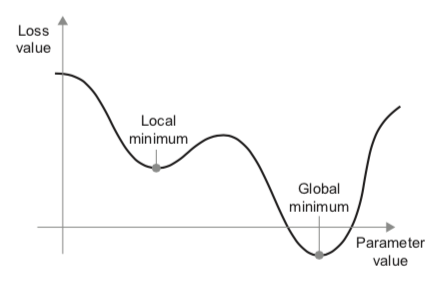
\includegraphics[width=.45\columnwidth]{../graphics/LocalGlobalMinimum}
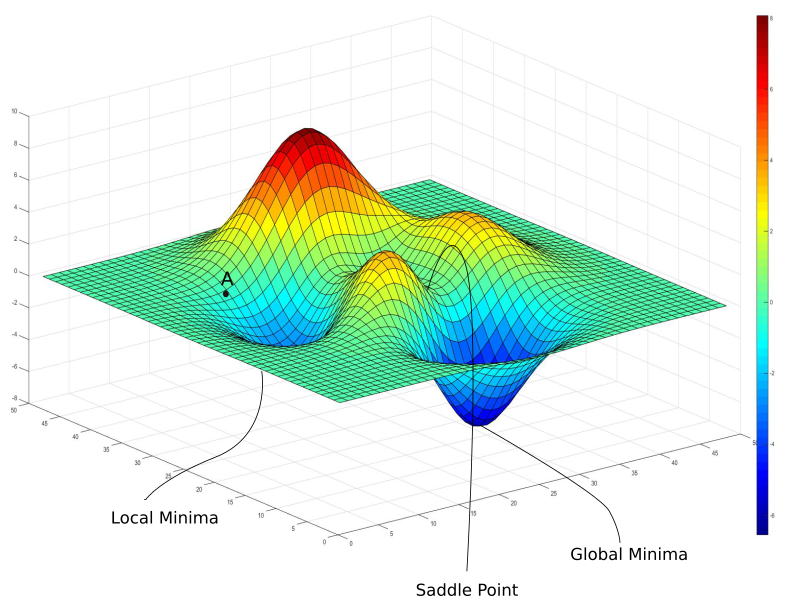
\includegraphics[width=.45\columnwidth]{../graphics/challenges1} \\
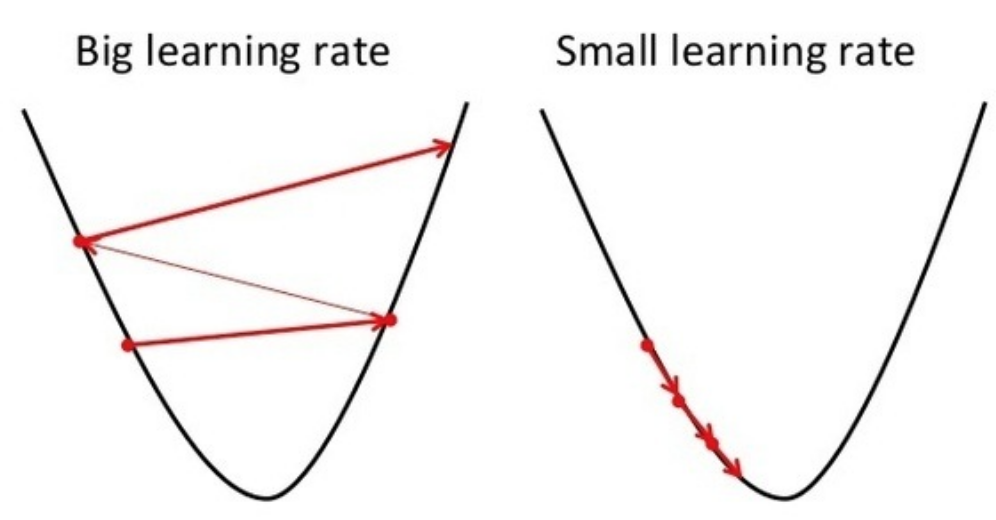
\includegraphics[width=.45\columnwidth]{../graphics/BigLearningRate}
\end{frame}

\begin{frame}
\begin{figure}
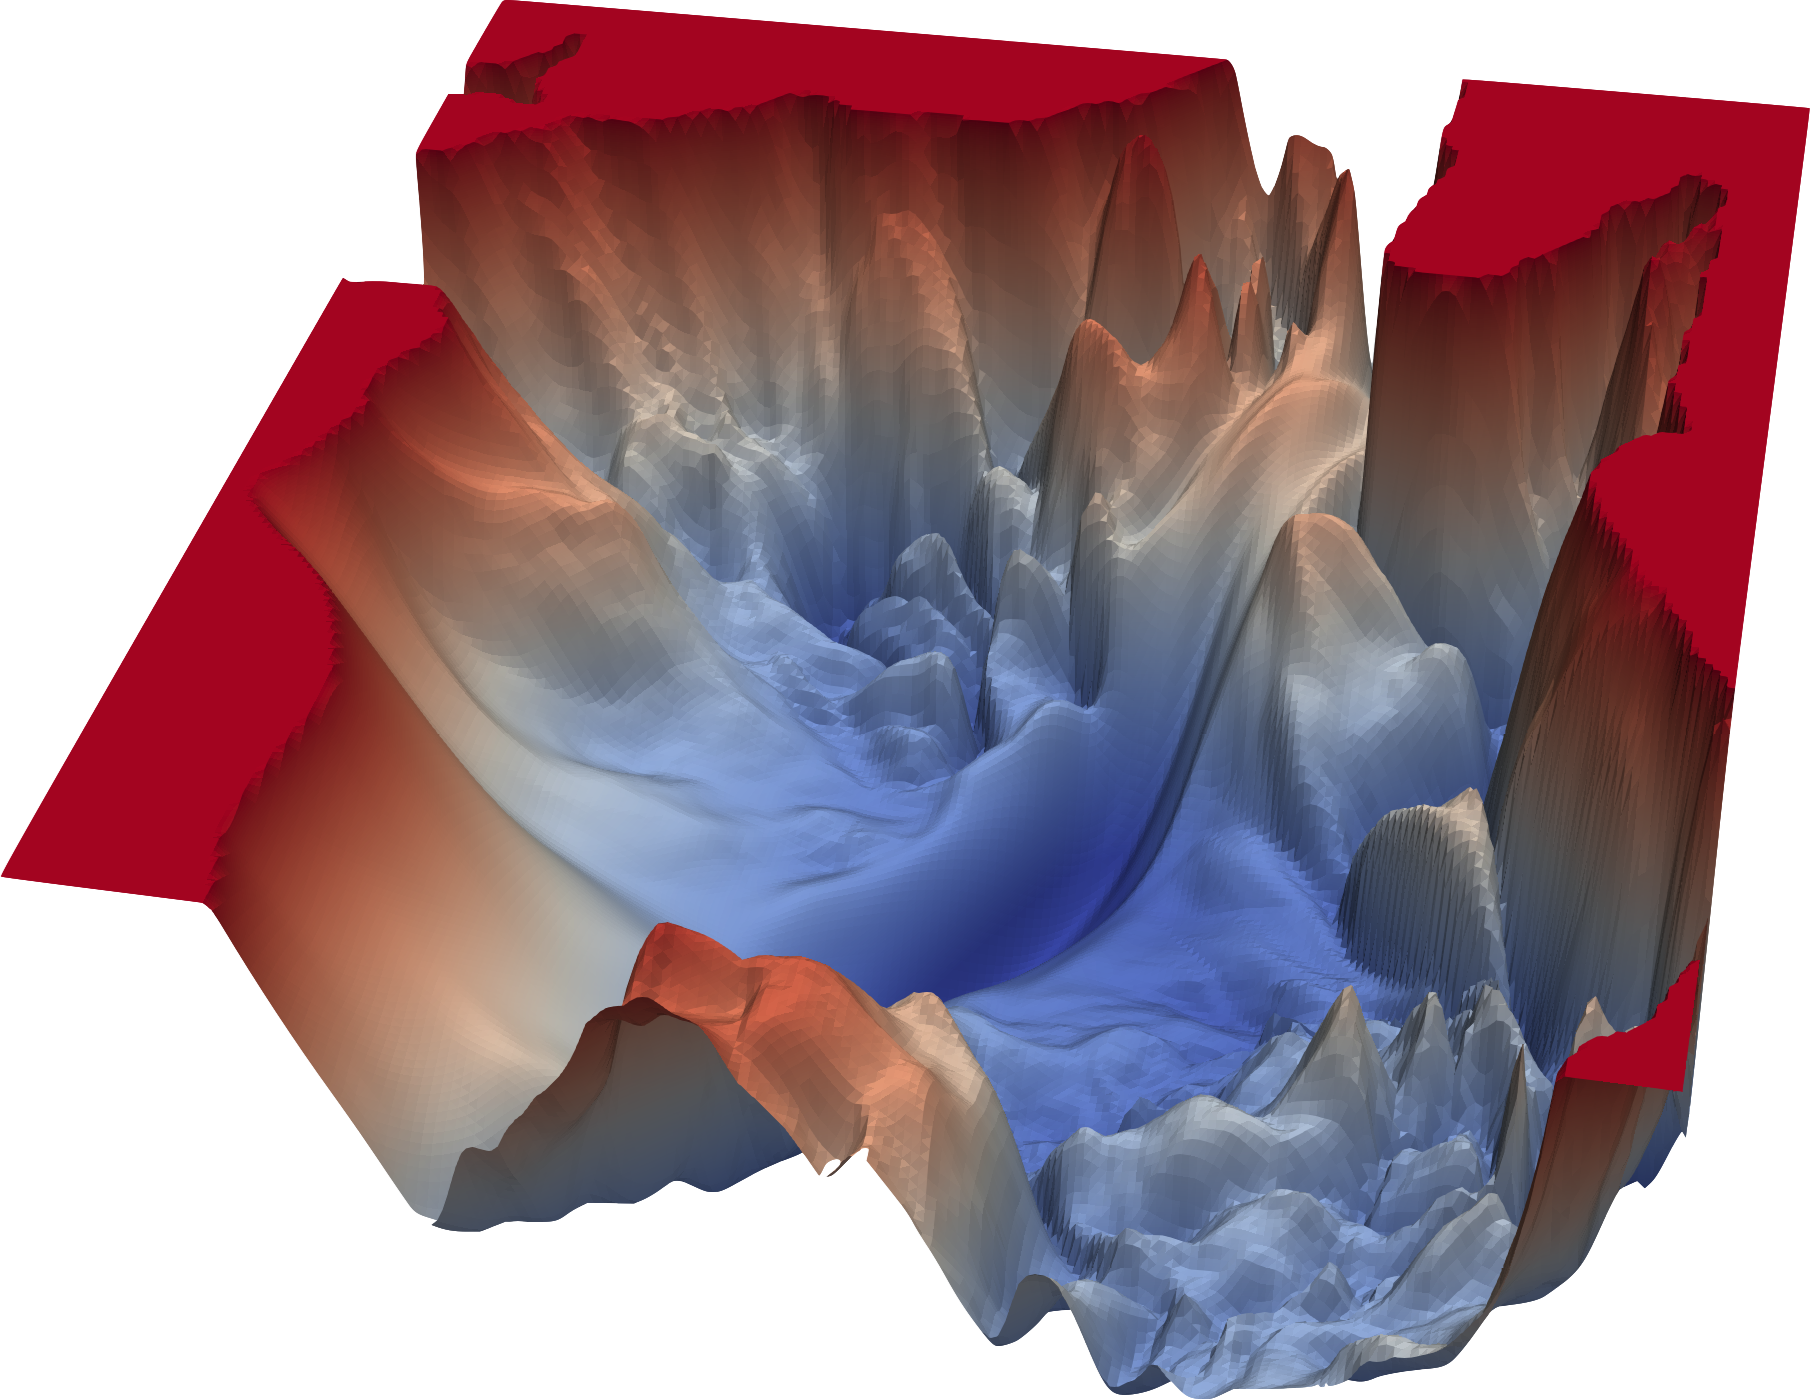
\includegraphics[width=.5\columnwidth]{../graphics/VGG56Loss}
\caption{Loss Function for VGG56}
\end{figure}
Reference: \textbf{Visualizing the Loss Landscape of Neural Net} \cite{li2017visualizing}
\end{frame}


\begin{frame}{Difficulties in Deep Network Optimisation}
\begin{itemize}
\item[C] {Vanishing Gradient:} If feedback signal has to be propagated through a deep stack of layers, the signal may become tenuous or even be lost entirely, rendering the network untrainable. During training, it causes the model's parameter to grow so large so that even a very tiny amount change in the input can cause a great update in later layers' output. The value of layer weights sometimes it overflow and the value becomes \alert{NaN}.
\end{itemize}
\end{frame}


\begin{frame}{Fighting against Vanishing Gradient}
\begin{enumerate}
\item[1] Initialization of Weights: Don't initialize to values that are too large.
\item[2] Gradient clipping: clips parameters gradients during backpropation by a maximum value or maximum norm 
\begin{figure}
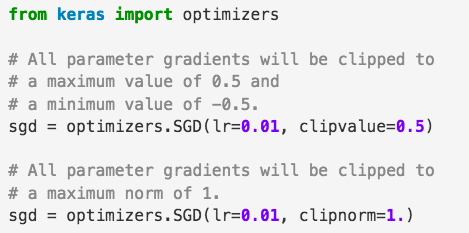
\includegraphics[width=.75\columnwidth]{../graphics/KerasClip}
\end{figure}
\end{enumerate}
On the difficulty of training Recurrent Neural Networks, \cite{pascanu2013difficulty}
\end{frame}

\begin{frame}{Fighting against Vanishing Gradient}
\begin{enumerate}
\item[3] Skip connections or Shortcuts (Residual Networks): 
\begin{figure}
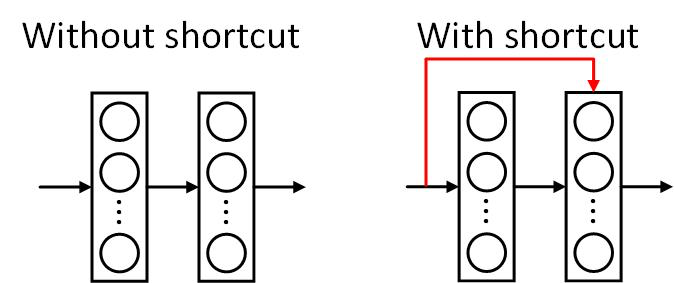
\includegraphics[width=.65 \columnwidth]{../graphics/shortcut}
\end{figure}
\end{enumerate}
\textbf{Visualizing the Loss Landscape of Neural Net}, \cite{li2017visualizing}

\end{frame}

\begin{frame}{Fighting against Vanishing Gradient}
\begin{enumerate}
\item[4] Avoid "stuck states" induced by activation function: 
\begin{figure}
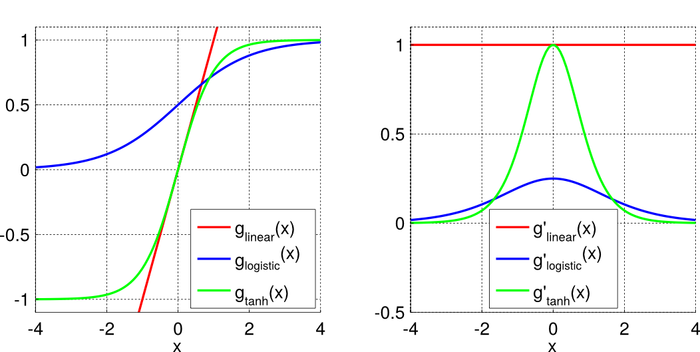
\includegraphics[width=.85 \columnwidth]{../graphics/nnet-error-functions2}
\caption{Left: Three activation function Right: Derivative of activation function.}
\end{figure}
\end{enumerate}
\end{frame}

\begin{frame}{Fighting against Vanishing Gradient}
\begin{enumerate}
\item[5] Regularization: $L_2$ or $L_1$ norm applies "weight decay" in the cost function of the network. Note that for many activation function, when the activation value is small, that will be almost linear.
\begin{figure}
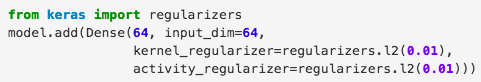
\includegraphics[width=.75 \columnwidth]{../graphics/KerasRegularizer}
\end{figure}

\end{enumerate}
\end{frame}


\begin{frame}{Batch Normalization}
TODO: FORMULA, EXAMPLES
\begin{eqnarray*}
\hat{x}_i = \frac{x_i-\mu_{B}}{\sqrt{\sigma^2_B}}\\
BN_{\gamma,\beta}(x_i):= \gamma \hat{x}_i + \beta
\end{eqnarray*}
where $\mu_{B}$ and $\sigma^2_B$ are respectively the mini-batch mean and variance. $\gamma$ scale and $\beta$ shift.
\begin{itemize}
\item In the original paper, BatchNorm is applied before the applying activation.
\item Moving values to zero (activation works better!) 
\item If we use a high learning rate in a traditional neural network, then the gradients could explode or vanish. Large learning rates can scale the parameters which could amplify the gradients, thus leading to an explosion. But if we do batch normalization, small changes in parameter to one layer do not get propagated to other layers. This makes it possible to use higher learning rates for the optimizers, which otherwise would not have been possible. It also makes gradient propagation in the network more stable.
\end{itemize}
\cite{ioffe2015batch}  \cite{mishkin2015all}
\end{frame}


%\begin{frame}
%\begin{itemize}
%\item[D]{Ill-conditioning of the Hessian Matrix}
%\end{itemize}
%\end{frame}

%%%%%%%%%%%%%%%%%%%%%%%%%%%%%%%%%%%%%%%%%%%%%%%%%%

\begin{frame}{Supervised Learning (Machine Learning)}
\begin{itemize}
\item \textbf{Data}: $\nsize$ observations $(\x_i,y_i) \in \mathcal{X} \times \mathcal{Y}, i=1,\ldots,\nsize$, \alert{\textbf{i.i.d.}}
\item \textbf{Model}: $\texttt{Model}(\x):=\param^T\featmap (\x)$ of features  $\featmap (\x) \in \mathbb{R}^\nfeatures$ \alert{Prediction as linear mapping of features}
\item \textbf{Minimization of Regularized Empirical Risk}: We would like to find $\param^{*}$ the solution of:
\begin{eqnarray*}
\param^{*}:=\min_{\param \in \mathbb{R}^\nfeatures} \frac{1}{\nsize} \sum_{i=1}^{\nsize} \loss(y_i,\param^T\featmap (\x))&  + &\alpha \mathcal{R}(\param) \\
\texttt{Data fitting}& + &\texttt{regularizer}
\end{eqnarray*}
\end{itemize}
where $\loss(\cdot,\cdot)$ is called the  \emph{loss function}.
\end{frame}



\begin{frame}{Other loss functions, other models}
%\begin{center}\includegraphics[width=.2\columnwidth]{../graphics/Loss}\end{center}
\begin{enumerate}
\item Support Vector Machine (SVM): "Hinge" Loss 
\begin{equation}
\loss(y,\param^T\featmap(\x))=\max \{1-y\param^T\featmap(\x),0\}
\end{equation}
\item Logistic Regression: 
\begin{equation}
\loss(y,\param^T\featmap(\x))=\log (1+\exp (-y\param^T\featmap(\x)))
\end{equation}
\item Mean Squared Regression:
\begin{equation}
\loss(y,\param^T\featmap(\x))=\frac{1}{2}(y-\param^T\featmap(\x))^2
\end{equation}
\item Adaboost
\begin{equation}
\loss(y,\param^T\featmap(\x))=\exp^{ -(y-\param^T\featmap(\x))}
\end{equation}
\item Others ...
\end{enumerate}
\end{frame}

\begin{frame}{Minimizing Empirial Risk = Problems!}
\begin{itemize}
\item Empirical Risk: $\hat{f}(\param) :=\frac{1}{\nsize} \sum_{i=1}^{\nsize} \loss(y_i,\param^T\featmap (\x_i))$ \pause \\\alert{Loss in a training set}
\end{itemize}
\begin{figure}[htb]
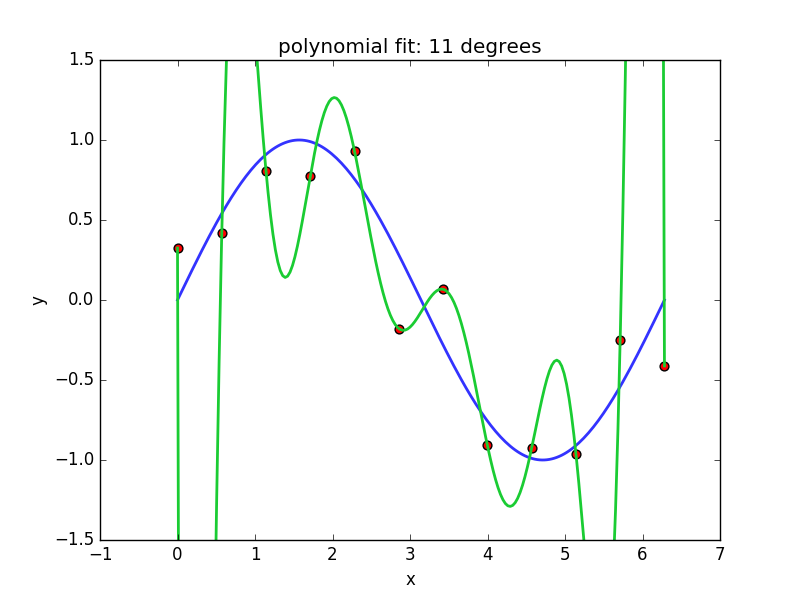
\includegraphics[width=0.6\textwidth]{../graphics/polyfit_degree_11.png}
%\caption{There are infinity minimizer of the empirical risk!}
\end{figure}
 \pause
\begin{itemize}
\item Expected Risk : $f(\param) := \mathbb{E}_{(\x,y)} \loss(y,\param^T\featmap (\x))$ \pause  \\\alert{Loss in a testing set}
\end{itemize}
There are infinity minimizers of the empirical risk, but most of them have a large expected risk (\alert{overfitting}).
\end{frame}


\section{How to fight against overfitting}

\begin{frame}{Bias/Variance Tradeoff}
Let $\hat{y}:=\texttt{Model}(\x)$ the prediction of a deterministic model evaluated at $\x$
\begin{eqnarray*}
\mathbb{E}_{(\x,y)}\left [ (y-\texttt{Model}(\x))^ 2\right ] = \\ Var\left[y \right] + Var \left[ \texttt{Model}(\x) \right] + (Bias [\texttt{Model}(\x)])^2
\end{eqnarray*}
\begin{figure}
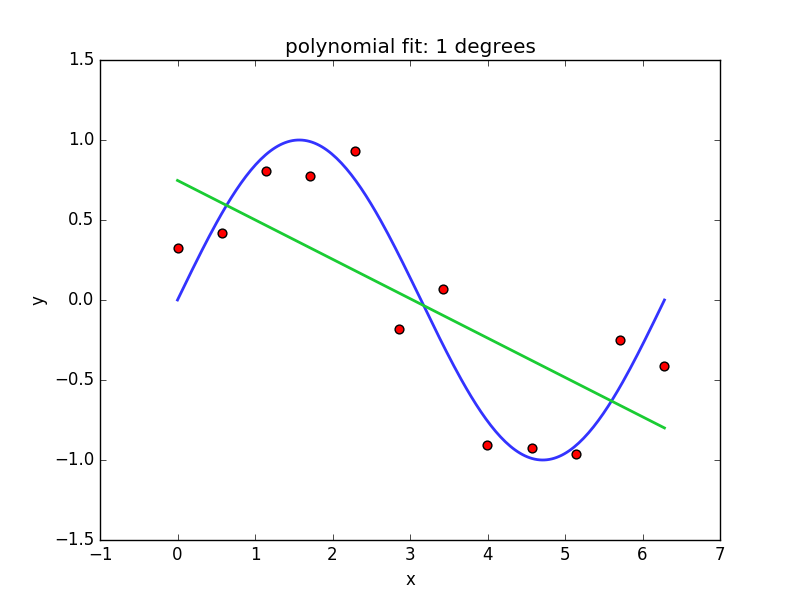
\includegraphics[width=.45 \columnwidth]{../graphics/polyfit_degree_1}
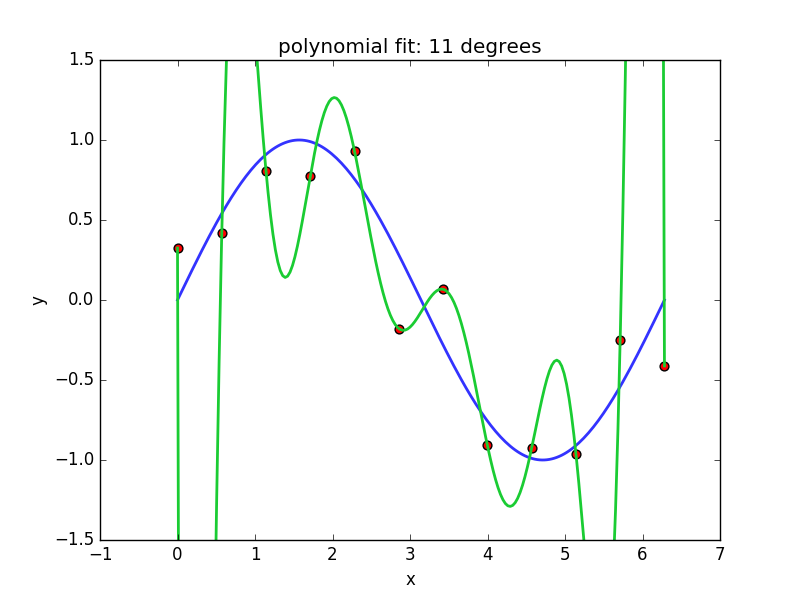
\includegraphics[width=.45 \columnwidth]{../graphics/polyfit_degree_11}
\caption{Underfitting / Overfitting}
\end{figure}
Underfitting : Prediction with less variance but more bias
Overfitting : Prediction with more variance but less bias
\end{frame}

\begin{frame}{How to judge if a deep machine learning model is overfitting or not?}
\begin{columns}
\begin{column}{.5\textwidth}
\includegraphics[width=.95 \columnwidth]{../graphics/overfitting}
\end{column}
\begin{column}{.5\textwidth}
\begin{itemize}
\item Training Set / Testing Set
\item Cross-Validation
\item $||\param||_p$ is large
\end{itemize}
\end{column}
\end{columns}
\end{frame}

\begin{frame}{1. Early Stopping / ReduceLROnPlateau / Learning Rate Scheduler}
\begin{figure}
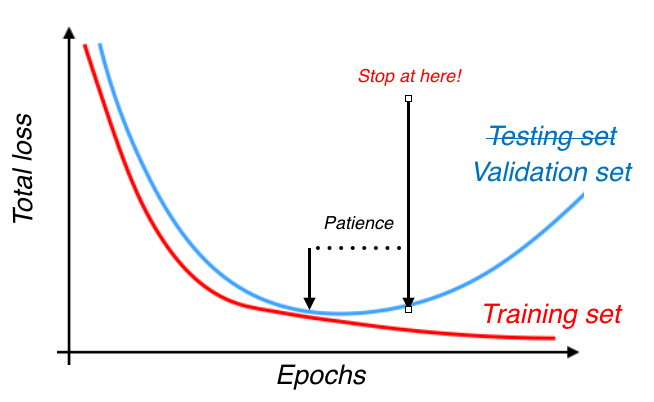
\includegraphics[width=.75 \columnwidth]{../graphics/EarlyStopping}
\end{figure}
\end{frame}

\begin{frame}{1. Early Stopping / ReduceLROnPlateau / Learning Rate Scheduler}
\begin{figure}
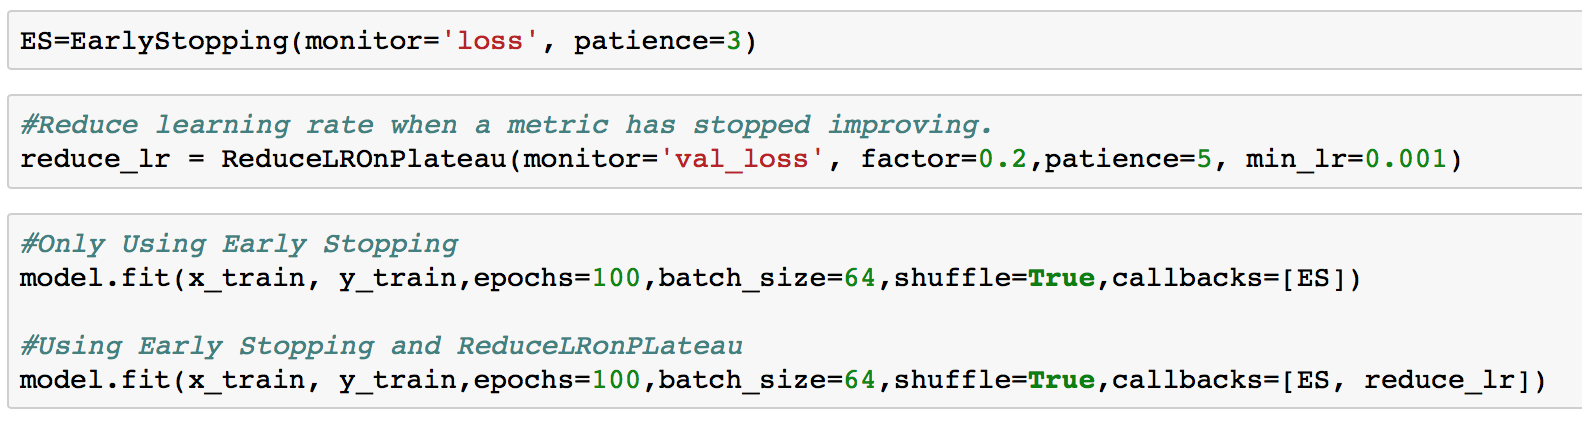
\includegraphics[width=1 \columnwidth]{../graphics/CallBacksKeras}
\caption{Callbacks in Keras}
\end{figure}
\end{frame}

\begin{frame}{2. We need more data!}
\begin{itemize}
\item Additive Gaussian noise.
\item Data augmentation.
\item Adversarial Training.
\end{itemize}
\end{frame}

\begin{frame}{Expected Risk (again)}
The expected risk
\begin{equation*}
 \mathbb{E}_{(\x,y)}  \loss(y,\texttt{Model}) =  \int \loss(y,\texttt{Model} (\x)) dP(\x,y) := R(\texttt{Model} )
\end{equation*}
\pause
But the distribution P is \alert{unknown} in most practical situations. 
\pause
We usually have access to a set of training data $T=\{(\x_i,y_i) \}_{i=1}^{\nsize}$, where $(\x_i,y_i)\sim P$, for all $i=1,\ldots,\nsize$. Thus, we may approximate $P$ by the \emph{empirical distribution}:
\begin{equation*}
P_{\delta}(\x,y) = \frac{1}{\nsize}\sum_{i=1}^{\nsize}\delta(\x=\x_i,y=y_i)
\end{equation*}
\end{frame}

\begin{frame}{Empirical Risk (again)}
Using the empirical distribution $P_{\delta}$, we can now approximated the expected risk, by the called \emph{empirical risk}
\begin{equation}\label{RM}
R_{\delta}(\texttt{Model} ) = \int \loss(y,\texttt{Model} (\x)) dP_{\alert{\delta}}(\x,y) = \frac{1}{\nsize}\sum_{i=1}^{\nsize}\loss(\texttt{Model}(\x_i),y_i)
\end{equation} \\
Learning the function $f$ by minimizing \eqref{RM} is known as the Empirical Risk Minimization (ERM) principle \cite{vapnik98} (Vapnik, 1998). If the number of parameters are comparable to $\nsize$, one trivial way to minimize \eqref{RM} is to \alert{memorize} the whole set of training data (overfitting).
\end{frame}

\begin{frame}{Vicinal Risk Minimization (VRM)}
$P_{\delta}$ is only one of the possibility to approximate the true distribution $P$. \cite{chapelle2001vicinal} proposed to approximate $P$ by:
\begin{equation*}
P_{v}(\x,y) = \frac{1}{\nsize}\sum_{i=1}^{\nsize}v(\tilde{\x},\tilde{y}, |\x_i,y_i)
\end{equation*}
where $v$ is \emph{vicinity distribution} that measure the probability for a "virtual" pair $(\tilde{\x},\tilde{y})$ to be in the \emph{vicinity} of the training pair $(\x,y)$. \pause
\begin{enumerate}
\item[1]  Gaussian vicinities: $v(\tilde{\x},\tilde{y}, |\x_i,y_i)=\mathcal{N}(\tilde{\x}-\x,\sigma^2\mathbf{I})\delta(\tilde{y}=y)$
\end{enumerate}
\pause
\alert{which is equivalent to augmenting the training data with additive Gaussian noise}
\end{frame}

\begin{frame}{Keras Gaussian Layer}
\begin{figure}
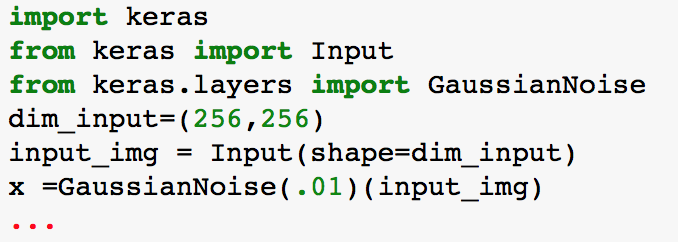
\includegraphics[width=.95 \columnwidth]{../graphics/GaussianNoiseLayer}
\caption{Gaussian vicinities in Keras}
\end{figure}
\end{frame}

\begin{frame}{Why Data-augmentation?}
\begin{enumerate}
\item[2]  Data-augmentation based vicinities: $P_{agg}(\x,y) = \frac{1}{\nsize}\sum_{i=1}^{\nsize}\delta(\tilde{\x},y_i)$, where $\tilde{\x}$ is a random transformation applied $\x$
\end{enumerate}
\begin{figure}
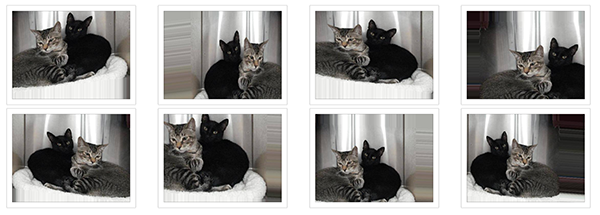
\includegraphics[width=.99 \columnwidth]{../graphics/cat_data_augmentation}
\caption{Example of a set of image produce by random transformations (translations, rotations, zooming, ...)}
\end{figure}
\end{frame}

\begin{frame}
\begin{figure}
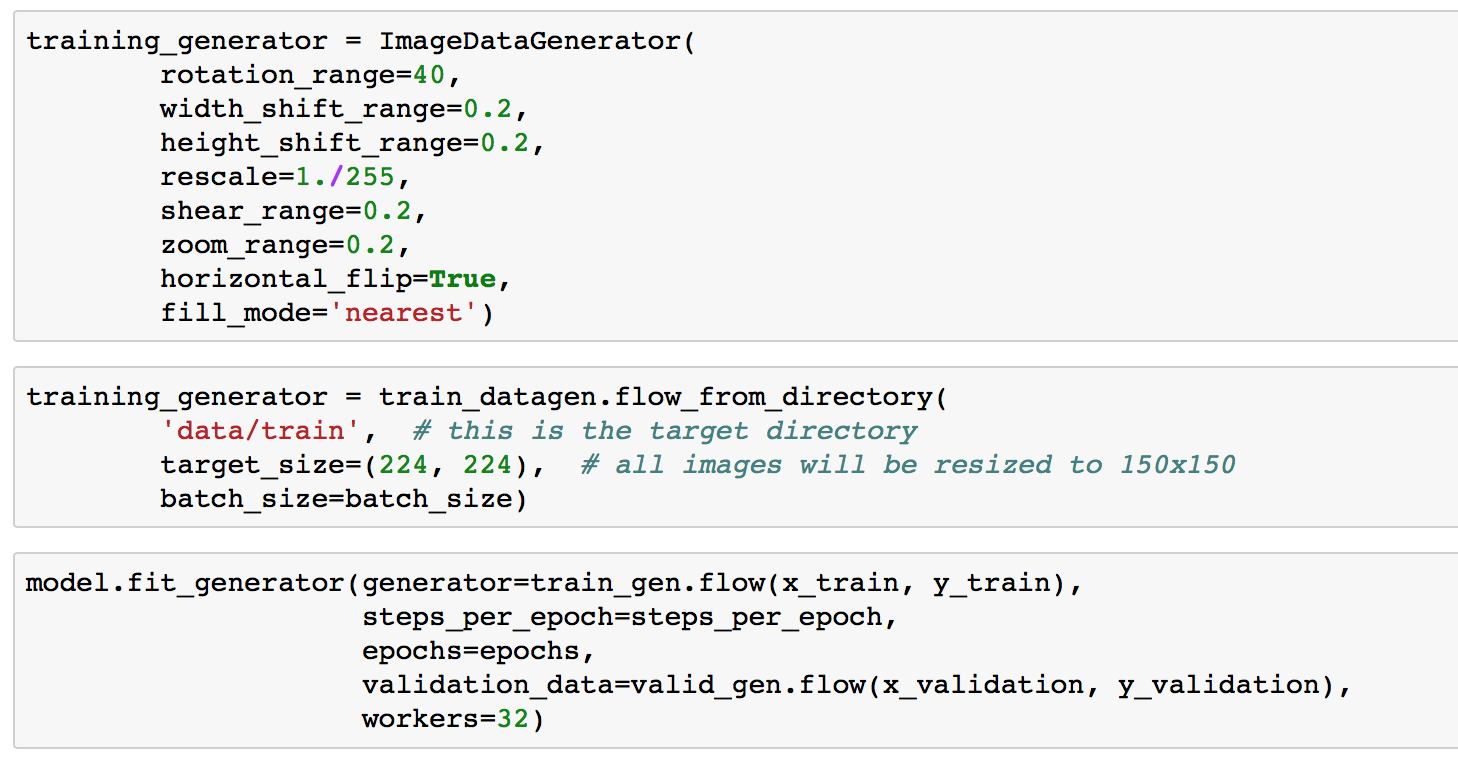
\includegraphics[width=.99 \columnwidth]{../graphics/DataGeneratorKeras}
\caption{Data Generator in Keras}
\end{figure}
\end{frame}

\begin{frame}{Regularisation}
\begin{enumerate}
\item "Weight Decay": Again?
\item Early Stopping
\item More data! : Data Augmentation
\item More data!  : Adversarial Examples
\item Summing-up: Dropout
\end{enumerate}
\end{frame}

\begin{frame}{How can we reduce the variance of ?}
\begin{itemize}
\item Remember: given $\nsize$ i.i.d. obsevations $\x_1,\x_2,\ldots,\x_\nsize$ each of them with variance equal to $\sigma^2$. 
\item What is the variance of $\bar{\x}=\frac{1}{\nsize} \sum_{i=1}^{\nsize} \x_i $? \pause $\frac{\sigma^2}{\nsize}$
\item \alert{Hint}: Train model on different training sets, and use the mean of predictions as final model of prediction.
\end{itemize}
\end{frame}

\begin{frame}{Dropout}
\begin{figure}
\includegraphics[width=.45 \columnwidth]{../graphics/NetworkDropoutNo}
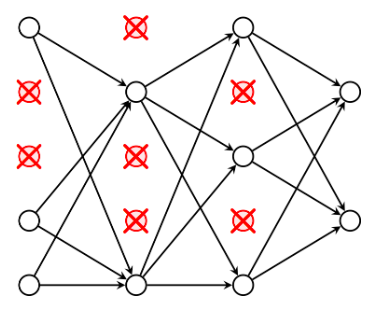
\includegraphics[width=.45 \columnwidth]{../graphics/NetworkDropoutYes}
\caption{Left: No Dropout Right: Dropout}
\end{figure}
\begin{itemize}
\item Since dropout can be seen as a stochastic regularization technique
\item Avoid memorization!
\item Dropout forces to learn more robust features that are useful in conjunction with many different random subsets.
\item With $H$ hidden units, each of which can be dropped, we have $2^H$ possible models!
\end{itemize}
Dropout: a simple way to prevent neural networks from overfitting. \cite{srivastava2014dropout} 2014
\end{frame}

\begin{frame}{Dropout}
\begin{figure}
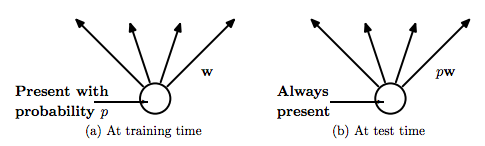
\includegraphics[width=.85 \columnwidth]{../graphics/DropoutP}
\caption{Left: A unit at training time that is present with probability $p$ and is connected to units
in the next layer with weights $\mathbf{w}$. Right: At test time, the unit is always present and
the weights are multiplied by $p$. The output at test time is same as the expected output
at training time.}
\end{figure}
\end{frame}


\begin{frame}{Dropout}
\begin{figure}
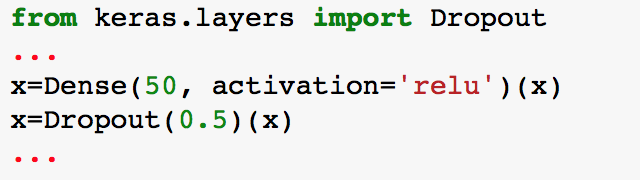
\includegraphics[width=.99 \columnwidth]{../graphics/DropoutKeras}
\caption{Dropout in Keras. Layer with a dropout of $p=.5$}
\end{figure}
\end{frame}
	
\begin{frame}{Initialization}
\begin{enumerate}
\item After the success of CNNs in IVSRC 2012 (\cite{krizhevsky2012imagenet}), initialization with Gaussian
noise with mean equal to zero and standard deviation set to 0.01 and adding bias equal to one
for some layers become very popular. But, as mentioned before, it is not possible to train very
deep network from scratch with it \cite{simonyan2014very}). The problem is caused by the
activation (and/or) gradient magnitude in final layers (\cite{he2016deep}).
% If each layer, not properly initialized, scales input by k, the final scale would be k L, where L is a number of layers.  
Values of $k > 1$ lead to extremely large values of output layers, $k < 1$ leads to a diminish
\item \cite{glorot2010understanding}  proposed a formula for estimating the standard deviation on the basis of
the number of input and output channels of the layers under assumption of no non-linearity between
layers. Despite invalidity of the assumption, Glorot initialization works well.	
\item Orthogonal : Independently, Saxe et al. \cite{saxe2013exact}  showed that orthonormal matrix initialization works much better
for linear networks than Gaussian noise, which is only approximate orthogonal. It also work for
networks with non-linearities.
\end{enumerate}
All you need is a good init, ICML, 2016 \cite{mishkin2015all}
\end{frame}

%%%%%%%%%%%%%%%%%%%%%%%%%%%%%%%%%%%%%%%%%%%%%%%%%%
%%%%%%%%%%%%%%%%%%%%%%%%%%%%%%%%%%%%%%%%%%%%%%%%%%
%%%%%%%%%%%%%%%%%%%%%%%%%%%%%%%%%%%%%%%%%%%%%%%%%%

\section{References}
\begin{frame}[allowframebreaks]
	\frametitle{References}
	\bibliography{slides_deep3.bib}
\end{frame}

\end{document}
